\documentclass[10pt]{article}
\usepackage[letterpaper,margin=1in]{geometry}
\usepackage{times}
\usepackage{microtype}
\usepackage{graphicx}
\usepackage{booktabs}
\usepackage{amsmath}
\usepackage[numbers,sort&compress]{natbib}
\usepackage[colorlinks=true,linkcolor=black,citecolor=blue,urlcolor=blue]{hyperref}

\title{Predictability is Trainable: Optimizing MoE LLMs to be Forecastable\\for Disk-Resident Inference}
\author{Spencer Churchill\\
Independent\\
\texttt{spence@duck.com}}
\date{}

\begin{document}
\maketitle

\begin{abstract}
Inference engines such as Colibr\`i run 744B-parameter Mixture-of-Experts
(MoE) models on consumer hardware by keeping the dense backbone resident and
streaming expert weights from disk on demand --- a reactive design whose
throughput is bounded by fetch latency. Post-hoc predictors can forecast
expert activations from earlier hidden states, but they chase a model never
asked to be predictable. We ask whether predictability is \emph{trainable}:
we fold the accuracy of a small expert-activation predictor into the MoE's
own training loss, so the model is optimized jointly for quality and for
being forecastable. At 341M-parameter scale we show that (i) predictability
is a trainable, transferable \textbf{backbone property} --- a fresh post-hoc
predictor on the frozen jointly-trained backbone recovers the full gain
(+6--7 pts top-$k$ hit rate over a linear control, +2.9--5.2 pts over a
ranking-aware control; both 3 seeds); (ii) the gain is \textbf{structural,
not sharpening} --- entropy penalties at any strength cannot reach it at
matched entropy; (iii) it \textbf{grows with training} while its quality
cost vanishes; and (iv) it converts to systems value (+3.2\% tok/s, $-$31\%
misprefetch waste in a disk-queue-accurate simulator; +5.0\% mean tok/s in a
purpose-built real engine). Finally we map the boundary: a LoRA fine-tune on
pretrained OLMoE-1B-7B transfers only a small fraction of the effect even at
10$\times$ loss pressure, indicating the method is
\textbf{pretraining-time only}.
\end{abstract}

\section{Introduction}

Sparse MoE LLMs activate only a small fraction of parameters per token, which
makes their \emph{weights} --- not their compute --- the binding resource on
consumer hardware. Engines like Colibr\`i \cite{colibri} exploit this: the
dense backbone stays resident while tens of thousands of routed experts are
streamed from disk, cached, and pinned by learned hot-stores. Every such
engine is reactive: the router fires, and only then does the fetch begin.
Colibr\`i's own mitigation is a router-lookahead thread (PILOT) that
prefetches next-layer experts, exploiting that routing is ${\sim}72\%$
predictable one layer ahead on a production model.

A literature of post-hoc predictors (\S\ref{sec:related}) shows expert
activations can be forecast from earlier hidden states with 93--97\%
accuracy. But all of it treats the model as fixed: the predictor chases the
model. We invert the relationship --- \textbf{the accuracy of an independent
expert-activation predictor becomes an explicit term in the MoE's own
training loss} --- so the backbone is regularized toward being forecastable
at multi-layer lookahead horizons while the predictor simultaneously adapts
to the model.\footnote{Code, data pipeline, run scripts, and the full audit
trail: \url{https://github.com/splch/predictability-aware-training}}

Contributions, each matched to an exhibit:
\begin{itemize}
\item \textbf{C1 --- Predictability is a trainable, transferable backbone
property.} Fresh post-hoc predictors trained on the frozen jointly-trained
backbone recover the entire gain; an engine needs no co-training to exploit
it (Table~\ref{tab:main}).
\item \textbf{C2 --- The gain is structural, not sharpening.} Entropy-penalty
controls at any strength cannot reach the jointly-trained predictability at
matched entropy; ${\sim}$+2--2.4 pts of the advantage is pure structure
(Figure~\ref{fig:frontier}).
\item \textbf{C3 --- The effect is robust and grows with training.} It
survives init + data-order variance ($\pm$0.3 pts) and \emph{increases} at
4$\times$ tokens, where the quality cost flips to a small gain
(Table~\ref{tab:robust}).
\item \textbf{C4 --- The accuracy converts to systems value, with a mapped
boundary.} +3.2\% tok/s and $-$31\% misprefetch waste over the post-hoc
control at Colibr\`i-like geometry (+1.6\%/$-$27\% at ranking-control
accuracies), gated by fetch\_time $\le$ compute\_window; +5.0\% mean tok/s
in a real O\_DIRECT engine; and a LoRA fine-tune on a pretrained model
recovers only a fraction of the effect even at 10$\times$ loss pressure ---
the method is pretraining-time only (Table~\ref{tab:tierc}).
\end{itemize}

\section{Related Work}
\label{sec:related}

\paragraph{Post-hoc expert prediction (frozen model).} Pre-attention linear
predictors with ranking-aware losses reach 93--97.6\% top-$k$ accuracy
\cite{zhu2025preattention}; cross-layer gate inputs enable edge offloading
with 99\% cache hits (Fate \cite{fang2025fate}); trace-trained sequence
predictors raise cache hit rates from 17\% to 72\% at 10\% budget
(MoE-Beyond \cite{gavhane2025moebeyond}); PreScope \cite{yu2025layerscope}
adds globally scheduled prefetching. Apple's LLM-in-a-Flash
\cite{alizadeh2023llmflash}, PowerInfer-2 \cite{xue2024powerinfer2}, and
MoE-Infinity \cite{xue2024moeinfinity} address adjacent offloading/caching
problems. All of these train predictors \emph{against} a fixed model; none
change the model.

\paragraph{Training-time routing modification.} StickyMoE
\cite{kayyam2026stickymoe} adds a differentiable routing-consistency loss
for temporal reuse --- the closest philosophy to ours, but it optimizes
\emph{stickiness} (token $t$ vs $t{-}1$), not \emph{forecastability from
earlier layers}; we show in \S\ref{sec:sticky} that it does not buy lookahead
predictability in our reimplementation. Oracle-MoE \cite{zhou2025oraclemoe}
redesigns the routing input for emergent locality (no explicit objective).
ReMoE \cite{zhu2026remoe} fine-tunes only the router post-hoc. Pre-gated MoE
\cite{hwang2024pregated} is the closest co-design: a pre-gate module that
\emph{replaces} next-layer routing, co-trained end-to-end with the backbone
--- but with no predictor-accuracy objective and no realized-router to
evaluate forecasts against. Halfway Speculative Decoding
\cite{nistor2026halfway} applies the same co-design pattern (train the
target to be draftable) in token space. Routing regularization for quality
or stability \cite{dai2022stablemoe,lv2025coupling,hu2026synergistic} never
targets inference-time predictability. No prior work, to our knowledge, adds
the accuracy of an \emph{independent} expert-activation predictor as an
explicit term in the MoE's own loss at multi-layer lookahead; our stronger
claim is empirical: that predictability is a transferable backbone property
(C1) with a structural signature distinguishable from entropy reduction (C2).

\paragraph{Our novelty statement, precisely scoped.} Prior systems work
trains predictors post-hoc against frozen models; prior training-time work
optimizes routing temporal locality; Pre-gated MoE co-trains a lookahead
gate that \emph{replaces} routing. We are aware of no work that (a) makes an
independent predictor's accuracy an explicit training objective of the MoE
itself, and (b) demonstrates the resulting predictability is a recoverable
property of the backbone's representations. Where this paper's ranking-aware
control reimplements \cite{zhu2025preattention}'s protocol, we say so; all
comparisons use our implementation, not their published numbers.

\section{Method}
\label{sec:method}

\paragraph{Model.} GPT-style decoder ($d{=}512$, 12 layers, 16 experts,
top-2, 341M total / 99M active parameters), trained on FineWeb-edu
\cite{penedo2024fineweb} (GPT-2 BPE \cite{radford2019gpt2},
document-shuffled stream with EOS, ctx 512, bf16 autocast).

\paragraph{Predictor.} Per-(layer, horizon) heads from the pre-MoE hidden
state at layer $l$ to the router decision at layer $l{+}h$,
$h \in \{1, 2, 4\}$. Two families: \emph{linear} (single projection) and
\emph{ranking-MLP} (2-layer MLP with a margin loss: the weakest true top-$k$
logit must exceed the strongest intruder by a margin), the latter
reimplementing the protocol of \cite{zhu2025preattention}.

\paragraph{Joint loss.} $L = L_{\mathrm{LM}} + 0.01 \cdot L_{\mathrm{balance}}
+ \lambda \cdot L_{\mathrm{pred}}$ (+ optional entropy or sticky terms for
controls). $L_{\mathrm{pred}}$ is a soft cross-entropy of predictor logits
against the realized top-$k$ set (uniform $1/k$ mass). Gradients from
$L_{\mathrm{pred}}$ reach the backbone only through hidden representations
(realized top-$k$ targets are argmax, non-differentiable) --- the loss shapes
representations, not router weights directly. The load-balancing term follows
Switch Transformer \cite{fedus2021switch}.

\paragraph{Isolation protocol (a first-class methodological contribution).}
To test whether predictability lives in the \emph{backbone} rather than in
predictor co-adaptation, we freeze a trained backbone and train a
\emph{fresh} predictor on it (2000--3000 steps), comparing against the same
fresh-predictor protocol on the baseline backbone. This mirrors deployment:
an inference engine trains its own predictor against a shipped model.

\paragraph{Metrics.} hit@$k$ per horizon (top-$k$ set overlap
$|\mathrm{pred} \cap \mathrm{true}| / k$); router entropy; adjacent-layer
routing persistence; utilization max; val LM loss on a fixed 16-batch
held-out set drawn once before training and shared by every run; zero-shot
downstream accuracy (HellaSwag \cite{zellers2019hellaswag}, ARC
\cite{clark2018arc}, PIQA \cite{bisk2020piqa}) scored by length-normalized
continuation logprob. Unless stated, numbers are $n{=}3$ seeds (init + data
order) with between-seed std.

\section{Experiments}
\label{sec:experiments}

\subsection{Setup and main result (Table~\ref{tab:main})}

Baseline ($\lambda{=}0$) vs joint ($\lambda{=}0.3$), 25M tokens, horizons
$\{1,2,4\}$. Controls are fresh post-hoc predictors on the frozen baseline
backbone; the joint row is the fresh-predictor-on-joint-backbone isolation
configuration.

\begin{table}[t]
\centering
\caption{hit@$k$ (between-seed std), fresh linear post-hoc predictor.
Chance = 0.125.}
\label{tab:main}
\begin{tabular}{lcccc}
\toprule
backbone & $h{=}1$ & $h{=}2$ & $h{=}4$ & val LM \\
\midrule
baseline & 0.826 (0.003) & 0.797 (0.002) & 0.732 (0.004) & 5.767 (0.006) \\
\textbf{joint ($\lambda{=}0.3$)} & \textbf{0.888 (0.002)} & \textbf{0.865 (0.002)} & \textbf{0.796 (0.004)} & 5.790 (0.006) \\
\bottomrule
\end{tabular}
\end{table}

Under the stronger ranking-MLP control (3 seeds): baseline 0.903 (0.001) /
0.865 (0.002) / 0.795 (0.001) vs joint \textbf{0.933 (0.002) / 0.907 (0.004)
/ 0.847 (0.008)} --- the advantage compresses to \textbf{+2.9 $\pm$ 0.2 /
+4.3 $\pm$ 0.3 / +5.2 $\pm$ 0.8 pts} (10--25$\times$ seed noise) but survives
intact under an identical predictor. We report +6--7 (linear) and +3--5
(ranking) as dual honest effect sizes throughout. Paired quality cost:
+0.023 $\pm$ 0.009 nats; +0.033 $\pm$ 0.016 with data-order variance
included.

\subsection{The isolation test (C1)}

A fresh post-hoc predictor on the frozen joint backbone recovers the
co-trained predictor's accuracy \emph{exactly} (0.890\slash 0.866\slash
0.796 vs 0.887\slash 0.863\slash 0.793). The predictability is a property of the weights --- the
deployable artifact.

\subsection{Structure, not sharpening (C2, Figure~\ref{fig:frontier})}

An entropy-penalty ladder ($\lambda_{\mathrm{ent}} \in \{0.005, 0.01,
0.05\}$) plus the baseline and joint points, all evaluated with the
ranking-MLP probe:

hit@1 vs entropy: baseline (2.26, 0.903) $<$ $\lambda 0.005$ (1.62, 0.912)
$<$ $\lambda 0.01$ (1.17, 0.916) $<$ \textbf{joint (2.10, 0.930)};
near-collapse (0.28) reaches only 0.883 under the linear probe.
Interpolating to the joint model's own entropy, sharpening alone yields
${\sim}$0.906--0.910: \textbf{${\sim}$+2.0--2.4 pts of the joint advantage
is pure structure} --- routing that is simultaneously informative and
forecastable, not merely peaked.

\begin{figure}[t]
\centering
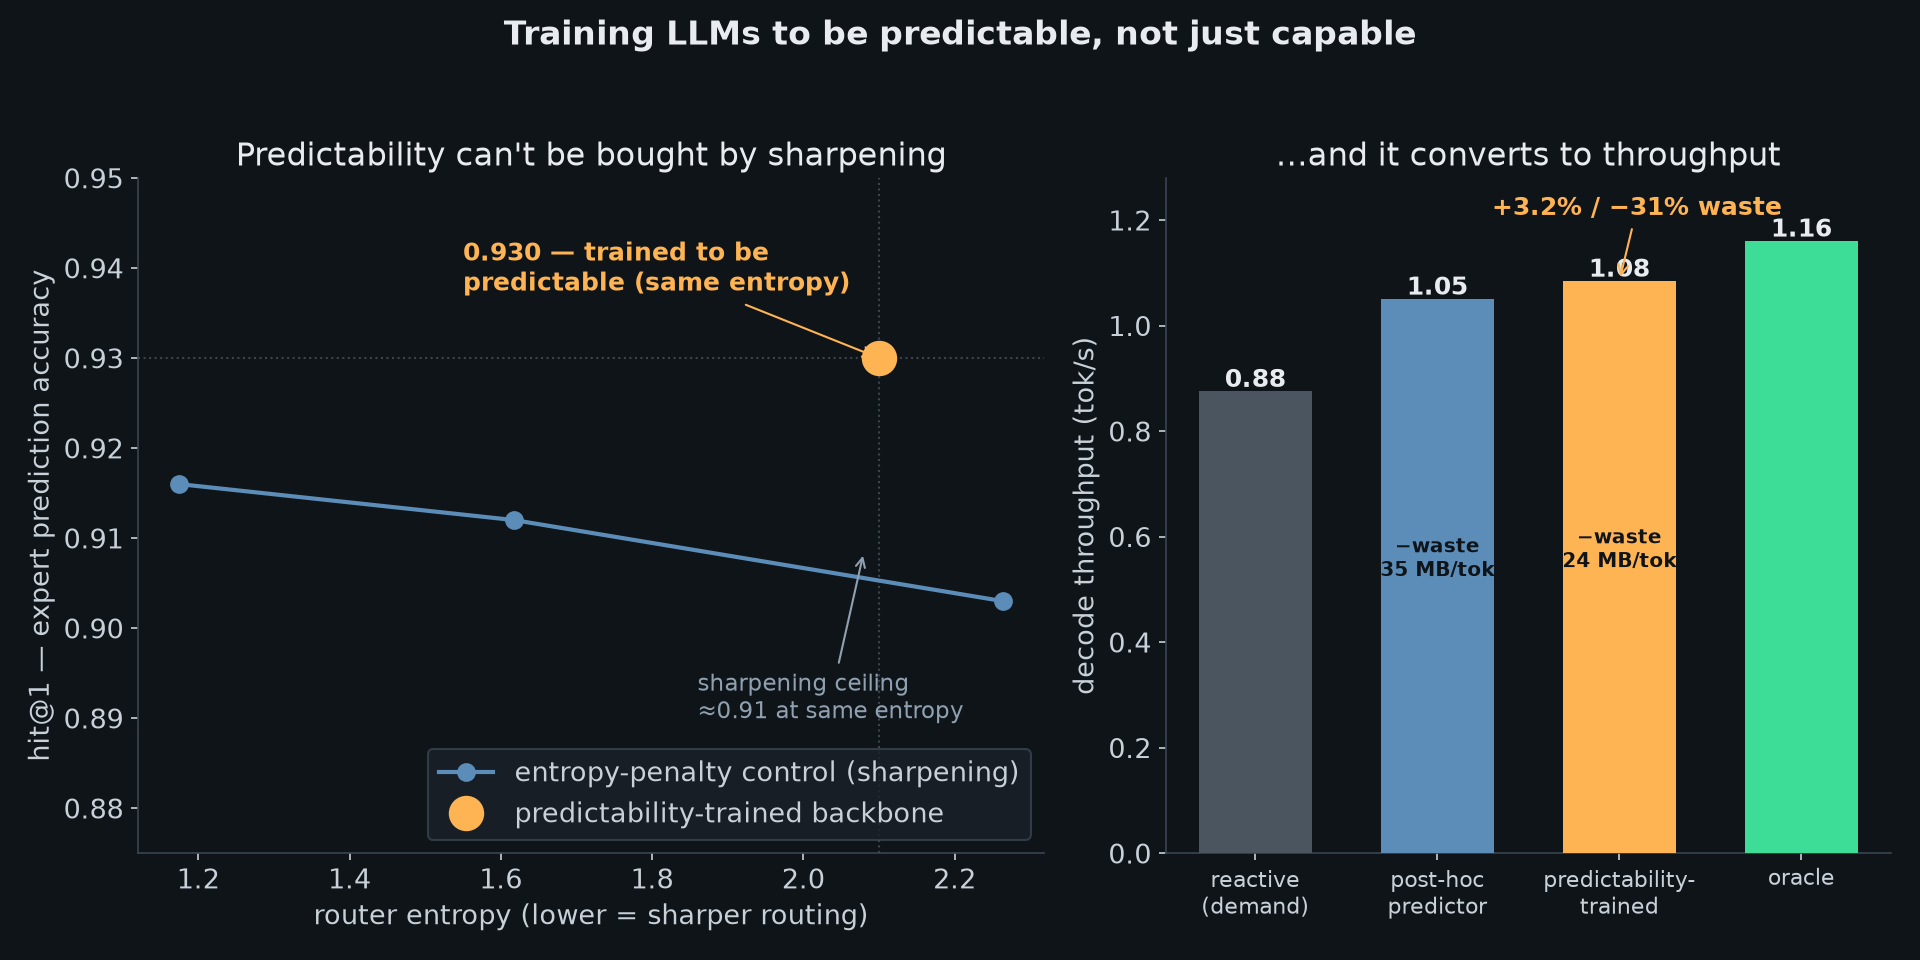
\includegraphics[width=\textwidth]{paper_figure.png}
\caption{(left) The entropy-penalty frontier plateaus at ${\sim}$0.91 hit@1
while the predictability-trained backbone reaches 0.930 at matched entropy;
(right) decode throughput and misprefetch waste at Colibr\`i-like geometry
(corrected simulator).}
\label{fig:frontier}
\end{figure}

\subsection{Robustness and growth with training (C3, Table~\ref{tab:robust})}

\begin{table}[t]
\centering
\caption{Robustness of the joint advantage across variance axes and training
length.}
\label{tab:robust}
\begin{tabular}{lcc}
\toprule
 & +hit@$k$ vs control ($h{=}1$ / $h{=}4$) & quality cost \\
\midrule
25M tokens, init-only variance & +6.2 $\pm$ 0.4 / +6.4 $\pm$ 0.6 & +0.023 $\pm$ 0.009 nats \\
25M tokens, init+data variance & +6.2 $\pm$ 0.3 / +6.8 $\pm$ 0.3 & +0.033 $\pm$ 0.016 nats \\
\textbf{100M tokens (4$\times$)} & \textbf{+6.1 / +7.9} & \textbf{$-$0.019 nats (free)} \\
\bottomrule
\end{tabular}
\end{table}

At 4$\times$ training the advantage \emph{grows} ($h4$ +7.9) and the quality
cost disappears; baseline routers sharpen naturally with training (entropy
2.26 $\to$ 1.98) and the joint model stays ahead. Zero-shot downstream
accuracy (HellaSwag/ARC-Easy/ARC-Challenge/PIQA, $n{=}1000$ each) is at
chance for both arms at 25M tokens (the model is too undertrained for task
sensitivity; paired deltas $-$0.6 $\pm$ 1.0 pp across 12 seed$\times$benchmark
pairs); at 100M tokens the joint model is at or above baseline on all four
benchmarks.

\subsection{Degeneracy checks}

At $\lambda{=}0.3$: entropy $-$9\% (no collapse), adjacent-layer persistence
$\approx$ chance (no temporal copying), utilization unchanged,
token-ID$\to$expert lookup probe equal in both backbones (no memorization),
marginal expert usage near-uniform (popularity trivial predictor hits 0.15).
At $\lambda{=}1.0$ the degenerate mode appears measurably: entropy $-$28\%
and +0.62 nats quality cost --- the frontier turns, visible in our
diagnostics.

\subsection{Training-time baseline: StickyMoE (Table~\ref{tab:sticky})}
\label{sec:sticky}

\begin{table}[t]
\centering
\caption{StickyMoE-style routing-consistency sweep (post-hoc linear probe on
each backbone). The consistency loss monotonically \emph{reduces} lookahead
predictability while raising router entropy.}
\label{tab:sticky}
\begin{tabular}{lccccc}
\toprule
arm & $h{=}1$ & $h{=}2$ & $h{=}4$ & entropy & val LM \\
\midrule
baseline & 0.822 & 0.791 & 0.724 & 2.264 & 5.949 \\
sticky 0.3 & 0.808 & 0.774 & 0.707 & 2.485 & 5.945 \\
sticky 1.0 & 0.793 & 0.754 & 0.682 & 2.599 & 5.957 \\
sticky 3.0 & 0.774 & 0.734 & 0.658 & 2.676 & 5.976 \\
\bottomrule
\end{tabular}
\end{table}

A routing-consistency loss (our reimplementation of StickyMoE's objective)
\emph{monotonically reduces} lookahead hit@$k$ while raising router entropy,
and does not stack with our loss (0.864 vs 0.884 joint-only). Scope: we
tested only lookahead predictability; StickyMoE's actual target ---
temporal-reuse cache locality --- is orthogonal and untested here.

\section{Systems Analysis}

\paragraph{Simulator.} A trace-driven engine with an honest single-disk FIFO
queue (demand-priority; prefetch issued only into idle compute windows that
fit the fetch; bandwidth conservation is exact). Synthetic Colibr\`i
geometry: 75$\times$256 experts, top-8, 19 MB int4 experts, 4 ms/layer dense
compute, $C{=}2000$-expert cache, Zipf+locality routing, predictor
accuracies measured in \S\ref{sec:experiments}.

\paragraph{Throughput (prefetch $h{=}1$).} demand 0.876 $\to$ base-control
1.051 $\to$ joint 1.085 $\to$ oracle 1.161 tok/s (linear-control
accuracies): \textbf{+3.2\% joint vs base, $-$31\% misprefetch waste (24.0
vs 34.6 MB/tok)}, ${\sim}$31\% of the base-to-oracle headroom captured. At
ranking-control accuracies (0.903 vs 0.933, 3-seed): \textbf{+1.6\% and
$-$27\% waste} --- the conversion paired with the honest effect size. TTFT
(cold cache): $-$11\% from prediction generally, $-$1--3\% joint vs base ---
not the differentiator.

\paragraph{Gating condition.} Across a 3$\times$3 latency/bandwidth grid the
joint-vs-base uplift is stable (+2.9--3.2\%) whenever prefetch fires; below
${\sim}$5 GB/s (19 MB expert), fetch time exceeds the compute window and
\emph{no} prefetch is possible: \textbf{bandwidth, not latency, gates the
regime} --- a design constraint for engines exploiting trained
predictability.

\paragraph{Real engine.} A purpose-built O\_DIRECT disk-resident engine for
the toy model (192 experts $\times$ 2.88 MB, demand-priority disk queue,
post-hoc predictor driving a prefetch thread, cache budget $C{=}64$): joint
vs base backbone, deployable configuration, 6 decode sequences:
\textbf{+5.0\% mean tok/s (range $-$7\% to +14.5\%)}, consistent with the
simulator's direction and magnitude; per-sequence variance is large at toy
scale, so we treat this as qualitative confirmation and keep the
quantitative claim on the simulator.

\section{Boundary: the method is pretraining-time (Table~\ref{tab:tierc})}

OLMoE-1B-7B \cite{muennighoff2024olmoe} (64 experts top-8, 3T pretraining
tokens), LoRA r16 on attention+experts plus trainable routers,
$\lambda \in \{0.1, 1.0\}$, 25M tokens:

\begin{table}[t]
\centering
\caption{Tier C isolation test on OLMoE-1B-7B (hit@$k$ at $h{=}1$/$h{=}2$/$h{=}4$).
At $\lambda{=}0.1$ the fine-tune leaves backbone predictability unchanged;
at 10$\times$ pressure a small transfer appears, still far weaker than
pretraining.}
\label{tab:tierc}
\begin{tabular}{lccc}
\toprule
post-hoc probe & on baseline backbone & on joint ($\lambda{=}0.1$) & on joint ($\lambda{=}1.0$) \\
\midrule
linear & 0.799 / 0.781 / 0.752 & 0.800 / 0.783 / 0.755 & 0.812 / 0.799 / 0.778 \\
ranking-MLP (177M) & 0.845 / 0.801 / 0.739 & 0.845 / 0.801 / 0.741 & 0.847 / 0.807 / 0.753 \\
\bottomrule
\end{tabular}
\end{table}

At the lower pressure ($\lambda{=}0.1$) the isolation test is a tie under
both probes. At 10$\times$ pressure ($\lambda{=}1.0$) a small backbone
effect appears --- +1.3/+1.8/+2.6 pts under the linear probe, +0.2/+0.6/+1.4
under the ranking probe, growing with horizon --- at +0.011 nats and with
router entropy flat (3.719 vs 3.748, so not sharpening). But this remains
\textbf{2.5--5$\times$ weaker than the pretraining effect under the linear
probe} (and more under the ranking probe, whose ceiling leaves less room):
the boundary is dose-dependent, not a strict zero, and the pretraining
regime is qualitatively different. We read this as \textbf{boundary mapping,
not failure}: representations must be shaped while plastic; the entire
training-time prior-art family (StickyMoE, Oracle-MoE) shares the property.
Scope of the negative: one seed, one LoRA rank, one token count (two
$\lambda$ values); heavier fine-tuning (unfrozen blocks, full FT) is
untested. Note also the baseline itself: a post-hoc predictor on stock OLMoE
reaches 0.845 $h{=}1$ --- post-hoc predictors are strong on real models, and
that is the bar any pretraining application must clear.

\section{Limitations}

Positive evidence is one toy from-scratch model (341M, 16 experts,
FineWeb-edu only, $\le$100M tokens); systems numbers are simulator +
toy-engine, not a production engine; quality is val-LM plus chance-level
zero-shot downstream probes (no consistent joint deficit at 25M tokens;
joint $\ge$ baseline on all four benchmarks at 100M tokens) --- task
sensitivity at this scale is limited; $n{=}3$; the ranking control is our
reimplementation of \cite{zhu2025preattention}'s protocol; StickyMoE was
tested on our metric only; the Tier C boundary rests on one seed / LoRA rank
/ token count (two $\lambda$ values). At toy $B{=}8$/$C{=}64$ the joint
engine row slightly exceeds the oracle (97.9 vs 97.4 tok/s) --- a
queue-interaction effect consistent with the waste ordering (oracle issues
more prefetch traffic), noted for completeness.

\section{Conclusion}

Predictability is trainable: an MoE optimized jointly for output quality and
for the accuracy of an independent expert-activation predictor becomes
measurably, structurally, and transferably more forecastable --- and the
gain converts to throughput and waste reductions wherever an engine has disk
slack. The effect must be baked in during pretraining. For pretraining labs
targeting disk-resident deployment, predictability pressure is a cheap
($\lambda \approx 0.3$), quality-neutral auxiliary objective; for engine
authors, the result defines what a shipped model can make recoverable. Data,
code, and the full audit trail (including three red-team rounds and all
negative results) are available in the repository:
\url{https://github.com/splch/predictability-aware-training}.

\bibliographystyle{plainnat}
\bibliography{references}

\end{document}
